% Created 2019-10-31 jeu. 09:48
% Intended LaTeX compiler: pdflatex
\documentclass[conference]{IEEEtran}
\usepackage[utf8]{inputenc}
\usepackage[T1]{fontenc}
\usepackage{graphicx}
\usepackage{grffile}
\usepackage{longtable}
\usepackage{wrapfig}
\usepackage{rotating}
\usepackage[normalem]{ulem}
\usepackage{amsmath}
\usepackage{textcomp}
\usepackage{amssymb}
\usepackage{capt-of}
\usepackage{hyperref}
\usepackage[most]{tcolorbox}
\usepackage{siunitx}
\IEEEoverridecommandlockouts
\usepackage{cite}
\usepackage{amsmath,amssymb,amsfonts}
\usepackage{algorithmic}
\usepackage{graphicx}
\usepackage{textcomp}
\usepackage{xcolor}
\usepackage{cases}
\usepackage{tabularx,siunitx,booktabs}
\usepackage{algorithmic}
\usepackage{import, hyperref}
\renewcommand{\citedash}{--}
\def\BibTeX{{\rm B\kern-.05em{\sc i\kern-.025em b}\kern-.08em T\kern-.1667em\lower.7ex\hbox{E}\kern-.125emX}}
\author{\IEEEauthorblockN{Dehaeze Thomas} \IEEEauthorblockA{\textit{European Synchrotron Radiation Facility} \\ Grenoble, France\\ \textit{Precision Mechatronics Laboratory} \\ \textit{University of Liege}, Belgium \\ thomas.dehaeze@esrf.fr }\and \IEEEauthorblockN{Verma Mohit} \IEEEauthorblockA{\textit{BEAMS Department}\\ \textit{Free University of Brussels}, Belgium\\ \textit{Precision Mechatronics Laboratory} \\ \textit{University of Liege}, Belgium \\ mohit.verma@ulb.ac.be }\and \IEEEauthorblockN{Collette Christophe} \IEEEauthorblockA{\textit{BEAMS Department}\\ \textit{Free University of Brussels}, Belgium\\ \textit{Precision Mechatronics Laboratory} \\ \textit{University of Liege}, Belgium \\ ccollett@ulb.ac.be }}
\date{2019-10-31}
\title{Complementary Filters Shaping \\ Using \(\mathcal{H}_\infty\) Synthesis \thanks{This work is funded by the FNRS.}}
\begin{document}

\maketitle


\bibliographystyle{IEEEtran}

\begin{abstract}
For many applications, large bandwidth and dynamic ranges are requiring to use several sensors, whose signals are combined using complementary filters.
This paper presents a method for designing these complementary filters using \(\mathcal{H}_\infty\) synthesis that allows to shape the filter norms.
This method is shown to be easily applicable for the synthesis of complex complementary filters.
\end{abstract}

\begin{IEEEkeywords}
Complementary Filters, Sensor Fusion, H-Infinity Synthesis
\end{IEEEkeywords}

\section{Introduction}
\label{sec:org88c7d86}
\label{sec:introduction}
A set of filters is said to be complementary if the sum of their transfer functions is equal to one at all frequencies.
These filters are used when two or more sensors are measuring the same physical quantity with different noise characteristics. Unreliable frequencies of each sensor are filtered out by the complementary filters and then combined to form a super sensor giving a better estimate of the physical quantity over a wider bandwidth.
This technique is called sensor fusion and is used in many applications.\par
In \cite{zimmermann92_high_bandw_orien_measur_contr,corke04_inert_visual_sensin_system_small_auton_helic,min15_compl_filter_desig_angle_estim}, various sensors (accelerometers, gyroscopes, vision sensors, etc.) are merged using complementary filters for the attitude estimation of Unmanned Aerial Vehicles (UAV).
In \cite{collette15_sensor_fusion_method_high_perfor}, several sensor fusion configurations using different types of sensors are discussed in order to increase the control bandwidth of active vibration isolation systems.
Furthermore, sensor fusion is used in the isolation systems of the Laser Interferometer Gravitational-Wave Observator (LIGO) to merge inertial sensors with relative sensors
\cite{matichard15_seism_isolat_advan_ligo,hua04_polyp_fir_compl_filter_contr_system}. \par
As the super sensor noise characteristics largely depend on the complementary filter norms, their proper design is of primary importance for sensor fusion.
In \cite{corke04_inert_visual_sensin_system_small_auton_helic,jensen13_basic_uas,min15_compl_filter_desig_angle_estim}, first and second order analytical formulas of complementary filters have been presented.
Higher order complementary filters have been used in
\cite{shaw90_bandw_enhan_posit_measur_using_measur_accel,zimmermann92_high_bandw_orien_measur_contr,collette15_sensor_fusion_method_high_perfor}.
In \cite{jensen13_basic_uas}, the sensitivity and complementary sensitivity transfer functions of a feedback architecture have been proposed to be used as complementary filters. The design of such filters can then benefit from the classical control theory developments.
Linear Matrix Inequalities (LMIs) are used in \cite{pascoal99_navig_system_desig_using_time} for the synthesis of complementary filters satisfying some frequency-like performance.
Finally, a synthesis method of high order Finite Impulse Response (FIR) complementary filters using convex optimization has been developed in \cite{hua05_low_ligo,hua04_polyp_fir_compl_filter_contr_system}. \par
Although many design methods of complementary filters have been proposed in the literature, no simple method that allows to shape the norm of the complementary filters is available.
This paper presents a new design method of complementary filters based on \(\mathcal{H}_\infty\) synthesis.
This design method permits to easily shape the norms of the generated filters.\par
The section \ref{sec:requirements} gives a brief overview of sensor fusion using complementary filters and explains how the typical requirements for such fusion can be expressed as upper bounds on the filters norms.
In section \ref{sec:hinf_method}, a new design method for the shaping of complementary filters using \(\mathcal{H}_\infty\) synthesis is proposed.
In section \ref{sec:application_ligo}, the method is used to design complex complementary filters that are used for sensor fusion at the LIGO.
Our conclusions are drawn in the final section.

\section{Complementary Filters Requirements}
\label{sec:org41613b0}
\label{sec:requirements}
\subsection{Sensor Fusion Architecture}
\label{sec:org3da9043}
\label{sec:sensor_fusion}

Let's consider two sensors measuring the same physical quantity \(x\) with dynamics \(G_1(s)\) and \(G_2(s)\), and with uncorrelated noise characteristics \(n_1\) and \(n_2\).

The signals from both sensors are fed into two complementary filters \(H_1(s)\) and \(H_2(s)\) and then combined to yield an estimate \(\hat{x}\) of \(x\) as shown in Fig. \ref{fig:fusion_super_sensor}.
\begin{equation}
\label{eq:comp_filter_estimate}
  \hat{x} = \left(G_1 H_1 + G_2 H_2\right) x + H_1 n_1 + H_2 n_2
\end{equation}

\begin{figure}[htbp]
\centering
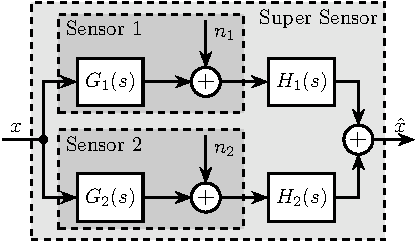
\includegraphics[scale=1]{figs/fusion_super_sensor.pdf}
\caption{\label{fig:fusion_super_sensor}
Sensor fusion architecture}
\end{figure}

The complementary property of \(H_1(s)\) and \(H_2(s)\) implies that their transfer function sum is equal to one at all frequencies \eqref{eq:comp_filter}.
\begin{equation}
\label{eq:comp_filter}
  H_1(s) + H_2(s) = 1
\end{equation}

\subsection{Noise Sensor Filtering}
\label{sec:org76c0d7c}
\label{sec:noise_filtering}

Let's first consider sensors with perfect dynamics
\begin{equation}
\label{eq:perfect_dynamics}
  G_1(s) = G_2(s) = 1
\end{equation}

The estimate \(\hat{x}\) is then described by
\begin{equation}
\label{eq:estimate_perfect_dyn}
  \hat{x} = x + H_1 n_1 + H_2 n_2
\end{equation}

From \eqref{eq:estimate_perfect_dyn}, the complementary filters \(H_1(s)\) and \(H_2(s)\) are shown to only operate on the sensor's noise.
Thus, this sensor fusion architecture permits to filter the noise of both sensors without introducing any distortion in the physical quantity to be measured.

Let's define the estimation error \(\delta x\) by \eqref{eq:estimate_error}.
\begin{equation}
\label{eq:estimate_error}
  \delta x \triangleq \hat{x} - x = H_1 n_1 + H_2 n_2
\end{equation}

As shown in \eqref{eq:noise_filtering_psd}, the Power Spectral Density (PSD) of the estimation error \(\Phi_{\delta x}\) depends both on the norm of the two complementary filters and on the PSD of the noise sources \(\Phi_{n_1}\) and \(\Phi_{n_2}\).
\begin{equation}
\label{eq:noise_filtering_psd}
  \Phi_{\delta x} = \left|H_1\right|^2 \Phi_{n_1} + \left|H_2\right|^2 \Phi_{n_2}
\end{equation}

Usually, the two sensors have high noise levels over distinct frequency regions.
In order to lower the noise of the super sensor, the value of the norm \(|H_1|\) has to be lowered when \(\Phi_{n_1}\) is larger than \(\Phi_{n_2}\) and that of \(|H_2|\) lowered when \(\Phi_{n_2}\) is larger than \(\Phi_{n_1}\).

\subsection{Robustness of the Fusion}
\label{sec:org60ae644}
\label{sec:fusion_robustness}

In practical systems the sensor dynamics is not perfect and \eqref{eq:perfect_dynamics} is not verified.
In such case, one can use an inversion filter \(\hat{G}_i^{-1}(s)\) to normalize the sensor dynamics, where \(\hat{G}_i(s)\) is an estimate of the sensor dynamics \(G_i(s)\).
However, as there is always some level of uncertainty on the dynamics, it cannot be perfectly inverted and \(\hat{G}_i^{-1}(s) G_i(s) \neq 1\).

Let's represent the resulting dynamic uncertainty of the inverted sensors by an input multiplicative uncertainty as shown in Fig. \ref{fig:sensor_fusion_dynamic_uncertainty} where \(\Delta_i\) is any stable transfer function satisfying \(|\Delta_i(j\omega)| \le 1,\ \forall\omega\), and \(|w_i(s)|\) is a weight representing the magnitude of the uncertainty.

\begin{figure}[htbp]
\centering
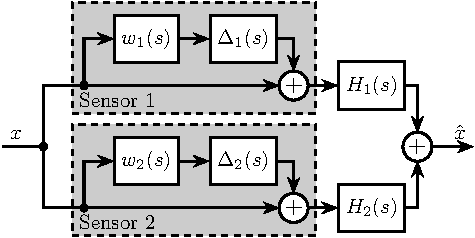
\includegraphics[scale=1]{figs/sensor_fusion_dynamic_uncertainty.pdf}
\caption{\label{fig:sensor_fusion_dynamic_uncertainty}
Sensor fusion architecture with sensor dynamics uncertainty}
\end{figure}

The super sensor dynamics \eqref{eq:super_sensor_dyn_uncertainty} is no longer equal to \(1\) and now depends on the sensor dynamics uncertainty weights \(w_i(s)\) as well as on the complementary filters \(H_i(s)\).
\begin{equation}
\label{eq:super_sensor_dyn_uncertainty}
  \frac{\hat{x}}{x} = 1 + w_1(s) H_1(s) \Delta_1(s) + w_2(s) H_2(s) \Delta_2(s)
\end{equation}

The uncertainty region of the super sensor can be represented in the complex plane by a circle centered on \(1\) with a radius equal to \(|w_1(j\omega) H_1(j\omega)| + |w_2(j\omega) H_2(j\omega)|\) as shown in Fig. \ref{fig:uncertainty_set_super_sensor}.

\begin{figure}[htbp]
\centering
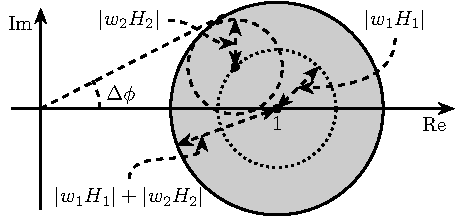
\includegraphics[scale=1]{figs/uncertainty_set_super_sensor.pdf}
\caption{\label{fig:uncertainty_set_super_sensor}
Uncertainty region of the super sensor dynamics in the complex plane (solid circle). The contribution of both sensors 1 and 2 to the uncertainty are represented respectively by a dotted and a dashed circle}
\end{figure}

The maximum phase added \(\Delta\phi(\omega)\) by the super sensor dynamics at frequency \(\omega\) is then
\begin{equation}
\label{eq:max_phase_uncertainty}
    \Delta\phi(\omega) = \arcsin\big( |w_1(j\omega) H_1(j\omega)| + |w_2(j\omega) H_2(j\omega)| \big)
\end{equation}

As it is generally desired to limit the maximum phase added by the super sensor, \(H_1(s)\) and \(H_2(s)\) should be designed such that \eqref{eq:max_uncertainty_super_sensor} is satisfied.
\begin{equation}
\label{eq:max_uncertainty_super_sensor}
   \max_\omega \big( \left|w_1 H_1\right| + \left|w_2 H_2\right|\big) < \sin\left( \Delta \phi_\text{max} \right)
\end{equation}
where \(\Delta \phi_\text{max}\) is the maximum allowed added phase.

Thus the norm of the complementary filter \(|H_i|\) should be made small at frequencies where \(|w_i|\) is large.

\section{Complementary Filters Shaping using \(\mathcal{H}_\infty\) Synthesis}
\label{sec:orgcafbd82}
\label{sec:hinf_method}
As shown in Sec. \ref{sec:requirements}, the performance and robustness of the sensor fusion architecture depends on the complementary filters norms.
Therefore, the development of a synthesis method of complementary filters that allows the shaping of their norm is necessary.
\subsection{Shaping of Complementary Filters using \(\mathcal{H}_\infty\) synthesis}
\label{sec:orga863dd2}
\label{sec:hinf_synthesis}
The synthesis objective is to shape the norm of two filters \(H_1(s)\) and \(H_2(s)\) while ensuring their complementary property \eqref{eq:comp_filter}.
This is equivalent as to finding stable transfer functions \(H_1(s)\) and \(H_2(s)\) such that conditions \eqref{eq:comp_filter_problem_form} are satisfied.
\begin{subequations}
\label{eq:comp_filter_problem_form}
  \begin{align}
  & H_1(s) + H_2(s) = 1 \label{eq:hinf_cond_complementarity} \\
  & |H_1(j\omega)| \le \frac{1}{|W_1(j\omega)|} \quad \forall\omega \label{eq:hinf_cond_h1} \\
  & |H_2(j\omega)| \le \frac{1}{|W_2(j\omega)|} \quad \forall\omega \label{eq:hinf_cond_h2}
  \end{align}
\end{subequations}
where \(W_1(s)\) and \(W_2(s)\) are two weighting transfer functions that are chosen to shape the norms of the corresponding filters.

In order to express this optimization problem as a standard \(\mathcal{H}_\infty\) problem, the architecture shown in Fig. \ref{fig:h_infinity_robust_fusion} is used where the generalized plant \(P\) is described by \eqref{eq:generalized_plant}.
\begin{equation}
\label{eq:generalized_plant}
  \begin{bmatrix} z_1 \\ z_2 \\ v \end{bmatrix} = P(s) \begin{bmatrix} w\\u \end{bmatrix}; \quad P(s) = \begin{bmatrix}W_1(s) & -W_1(s) \\ 0 & W_2(s) \\  1 & 0 \end{bmatrix}
\end{equation}

\begin{figure}[htbp]
\centering
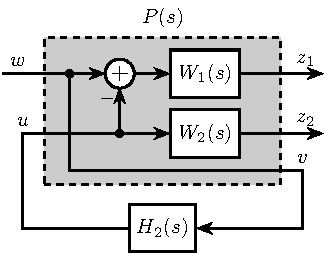
\includegraphics[scale=1]{figs/h_infinity_robust_fusion.pdf}
\caption{\label{fig:h_infinity_robust_fusion}
Architecture used for \(\mathcal{H}_\infty\) synthesis of complementary filters}
\end{figure}

The \(\mathcal{H}_\infty\) filter design problem is then to find a stable filter \(H_2(s)\) which based on \(v\), generates a signal \(u\) such that the \(\mathcal{H}_\infty\) norm from \(w\) to \([z_1, \ z_2]\) is less than one \eqref{eq:hinf_syn_obj}.
\begin{equation}
\label{eq:hinf_syn_obj}
  \left\|\begin{matrix} \left[1 - H_2(s)\right] W_1(s) \\ H_2(s) W_2(s) \end{matrix}\right\|_\infty \le 1
\end{equation}

This is equivalent to having \eqref{eq:hinf_problem} by defining \(H_1(s)\) as the complementary filter of \(H_2(s)\) \eqref{eq:definition_H1}.
\begin{equation}
\label{eq:hinf_problem}
  \left\|\begin{matrix} H_1(s) W_1(s) \\ H_2(s) W_2(s) \end{matrix}\right\|_\infty \le 1
\end{equation}

\begin{equation}
\label{eq:definition_H1}
  H_1(s) \triangleq 1 - H_2(s)
\end{equation}

The complementary condition \eqref{eq:hinf_cond_complementarity} is ensured by \eqref{eq:definition_H1}.
The conditions \eqref{eq:hinf_cond_h1} and \eqref{eq:hinf_cond_h2} on the filters shapes are satisfied by \eqref{eq:hinf_problem}.
Therefore, all the conditions \eqref{eq:comp_filter_problem_form} are satisfied using this synthesis method based on \(\mathcal{H}_\infty\) synthesis, and thus it permits to shape complementary filters as desired.

\subsection{Weighting Functions Design}
\label{sec:orgfe75ec2}
\label{sec:hinf_weighting_func}
The proper design of the weighting functions is of primary importance for the success of the presented complementary filters \(\mathcal{H}_\infty\) synthesis.

First, only proper, stable and minimum phase transfer functions should be used.
Second, the order of the weights should stay reasonably small in order to reduce the computational costs associated with the solving of the optimization problem and for the physical implementation of the filters (the order of the synthesized filters being equal to the sum of the weighting functions order).
Third, one should not forget the fundamental limitations imposed by the complementary property \eqref{eq:comp_filter}.
This implies for instance that \(|H_1(j\omega)|\) and \(|H_2(j\omega)|\) cannot be made small at the same time.

When designing complementary filters, it is usually desired to specify the slope of the filter, its crossover frequency and its gain at low and high frequency.
To help with the design of the weighting functions such that the above specification can be easily expressed, the following formula is proposed.
\begin{equation}
\label{eq:weight_formula}
  W(s) = \left( \frac{
           \hfill{} \frac{1}{\omega_0} \sqrt{\frac{1 - \left(\frac{G_0}{G_c}\right)^{\frac{2}{n}}}{1 - \left(\frac{G_c}{G_\infty}\right)^{\frac{2}{n}}}} s + \left(\frac{G_0}{G_c}\right)^{\frac{1}{n}}
         }{
           \left(\frac{1}{G_\infty}\right)^{\frac{1}{n}} \frac{1}{\omega_0} \sqrt{\frac{1 - \left(\frac{G_0}{G_c}\right)^{\frac{2}{n}}}{1 - \left(\frac{G_c}{G_\infty}\right)^{\frac{2}{n}}}} s + \left(\frac{1}{G_c}\right)^{\frac{1}{n}}
         }\right)^n
\end{equation}
The parameters permit to specify:
\begin{itemize}
\item the low frequency gain: \(G_0 = lim_{\omega \to 0} |W(j\omega)|\)
\item the high frequency gain: \(G_\infty = lim_{\omega \to \infty} |W(j\omega)|\)
\item the absolute gain at \(\omega_0\): \(G_c = |W(j\omega_0)|\)
\item the absolute slope between high and low frequency: \(n\)
\end{itemize}

The parameters \(G_0\), \(G_c\) and \(G_\infty\) should either satisfy condition \eqref{eq:cond_formula_1} or \eqref{eq:cond_formula_2}.
\begin{subequations}
\label{eq:condition_params_formula}
  \begin{align}
    G_0 < 1 < G_\infty \text{ and } G_0 < G_c < G_\infty \label{eq:cond_formula_1}\\
    G_\infty < 1 < G_0 \text{ and } G_\infty < G_c < G_0 \label{eq:cond_formula_2}
  \end{align}
\end{subequations}

The general shape of a weighting function generated using \eqref{eq:weight_formula} is shown in Fig. \ref{fig:weight_formula}.

\begin{figure}[htbp]
\centering
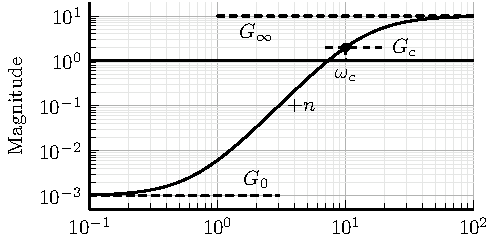
\includegraphics[scale=1]{figs/weight_formula.pdf}
\caption{\label{fig:weight_formula}
Magnitude of a weighting function generated using the proposed formula \eqref{eq:weight_formula}, \(G_0 = 1e^{-3}\), \(G_\infty = 10\), \(\omega_c = \SI{10}{Hz}\), \(G_c = 2\), \(n = 3\)}
\end{figure}

\subsection{Validation of the proposed synthesis method}
\label{sec:org0bf5120}
\label{sec:hinf_example}
Let's validate the proposed design method of complementary filters with a simple example where two complementary filters \(H_1(s)\) and \(H_2(s)\) have to be designed such that:
\begin{itemize}
\item the merging frequency is around \(\SI{10}{Hz}\)
\item the slope of \(|H_1(j\omega)|\) is \(-2\) above \(\SI{10}{Hz}\)
\item the slope of \(|H_2(j\omega)|\) is \(+3\) below \(\SI{10}{Hz}\)
\item the gain of both filters is equal to \(10^{-3}\) away from the merging frequency
\end{itemize}

The weighting functions \(W_1(s)\) and \(W_2(s)\) are designed using \eqref{eq:weight_formula}.
The parameters used are summarized in table \ref{tab:weights_params} and the magnitude of the weighting functions is shown in Fig. \ref{fig:hinf_synthesis_results}.

\begin{table}[htbp]
\caption{\label{tab:weights_params}
Parameters used for \(W_1(s)\) and \(W_2(s)\)}
\centering
\begin{tabularx}{0.5\linewidth}{Xcc}
\toprule
Parameter & \(W_1(s)\) & \(W_2(s)\)\\
\midrule
\(G_0\) & \(0.1\) & \(1000\)\\
\(G_\infty\) & \(1000\) & \(0.1\)\\
\(\omega_c\) [\(\si{Hz}\)] & \(11\) & \(10\)\\
\(G_c\) & \(0.5\) & \(0.5\)\\
\(n\) & \(2\) & \(3\)\\
\bottomrule
\end{tabularx}
\end{table}

The bode plots of the obtained complementary filters are shown in Fig. \ref{fig:hinf_synthesis_results} and their transfer functions in the Laplace domain are given below.
\begin{align*}
  H_1(s) &= \frac{10^{-8} (s+6.6e^9) (s+3450)^2 (s^2 + 49s + 895)}{(s+6.6e^4) (s^2 + 106 s + 3e^3) (s^2 + 72s + 3580)}\\
  H_2(s) &= \frac{(s+6.6e^4) (s+160) (s+4)^3}{(s+6.6e^4) (s^2 + 106 s + 3e^3) (s^2 + 72s + 3580)}
\end{align*}

\begin{figure}[htbp]
\centering
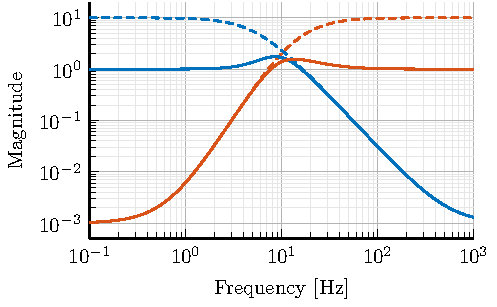
\includegraphics[scale=1]{figs/hinf_synthesis_results.pdf}
\caption{\label{fig:hinf_synthesis_results}
Frequency response of the weighting functions and complementary filters obtained using \(\mathcal{H}_\infty\) synthesis}
\end{figure}

\subsection{Synthesis of Three Complementary Filters}
\label{sec:org9751f7b}
\label{sec:hinf_three_comp_filters}
Some applications may require to merge more than two sensors.
In such a case, it is necessary to design as many complementary filters as the number of sensors used.
The synthesis problem is then to compute \(n\) stable transfer functions \(H_i(s)\) such that \eqref{eq:hinf_problem_gen} is satisfied.
\begin{subequations}
\label{eq:hinf_problem_gen}
  \begin{align}
  & \sum_{i=0}^n H_i(s) = 1 \label{eq:hinf_cond_compl_gen} \\
  & \left| H_i(j\omega) \right| < \frac{1}{\left| W_i(j\omega) \right|}, \quad \forall \omega,\ i = 1 \dots n \label{eq:hinf_cond_perf_gen}
  \end{align}
\end{subequations}
The synthesis method is generalized here for the synthesis of three complementary filters using the architecture shown in Fig. \ref{fig:comp_filter_three_hinf}.

The \(\mathcal{H}_\infty\) synthesis objective applied on \(P(s)\) is to design two stable filters \(H_2(s)\) and \(H_3(s)\) such that the \(\mathcal{H}_\infty\) norm of the transfer function from \(w\) to \([z_1,\ z_2, \ z_3]\) is less than one \eqref{eq:hinf_syn_obj_three}.
\begin{equation}
\label{eq:hinf_syn_obj_three}
  \left\| \begin{matrix} \left[1 - H_2(s) - H_3(s)\right] W_1(s) \\ H_2(s) W_2(s) \\ H_3(s) W_3(s) \end{matrix} \right\|_\infty \le 1
\end{equation}

\begin{figure}[htbp]
\centering
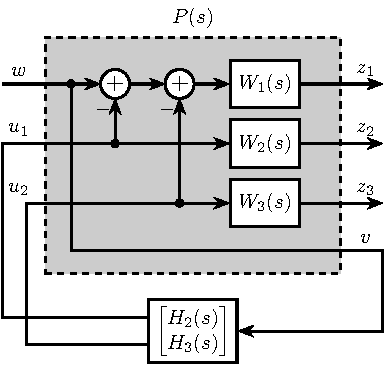
\includegraphics[scale=1]{figs/comp_filter_three_hinf.pdf}
\caption{\label{fig:comp_filter_three_hinf}
Architecture for \(\mathcal{H}_\infty\) synthesis of three complementary filters}
\end{figure}

By choosing \(H_1(s) \triangleq 1 - H_2(s) - H_3(s)\), the proposed \(\mathcal{H}_\infty\) synthesis solves the design problem \eqref{eq:hinf_problem_gen}. \par
An example is given to validate the method where three sensors are used in different frequency bands (up to \(\SI{1}{Hz}\), from \(1\) to \(\SI{10}{Hz}\) and above \(\SI{10}{Hz}\) respectively).
Three weighting functions are designed using \eqref{eq:weight_formula} and shown by dashed curves in Fig. \ref{fig:hinf_three_synthesis_results}.
The bode plots of the obtained complementary filters are shown in Fig. \ref{fig:hinf_three_synthesis_results}.

\begin{figure}[htbp]
\centering
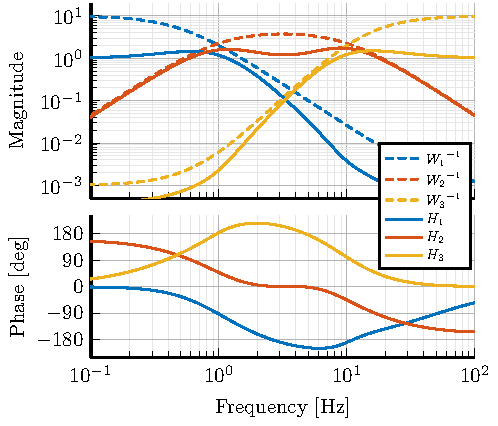
\includegraphics[scale=1]{figs/hinf_three_synthesis_results.pdf}
\caption{\label{fig:hinf_three_synthesis_results}
Frequency response of the weighting functions and three complementary filters obtained using \(\mathcal{H}_\infty\) synthesis}
\end{figure}

\section{Application: Design of Complementary Filters used in the Active Vibration Isolation System at the LIGO}
\label{sec:orgc2ed648}
\label{sec:application_ligo}
Several complementary filters are used in the active isolation system at the LIGO \cite{hua05_low_ligo,hua04_polyp_fir_compl_filter_contr_system}.
The requirements on those filters are very tight and thus their design is complex.
The approach used in \cite{hua05_low_ligo} for their design is to write the synthesis of complementary FIR filters as a convex optimization problem.
The obtained FIR filters are compliant with the requirements. However they are of very high order so their implementation is quite complex.

The effectiveness of the proposed method is demonstrated by designing complementary filters with the same requirements as the one described in \cite{hua05_low_ligo}.
\subsection{Complementary Filters Specifications}
\label{sec:orgfeebf2a}
\label{sec:ligo_specifications}
The specifications for one pair of complementary filters used at the LIGO are summarized below (for further details, refer to \cite{hua04_polyp_fir_compl_filter_contr_system}) and shown in Fig. \ref{fig:ligo_weights}:
\begin{itemize}
\item From \(0\) to \(\SI{0.008}{Hz}\), the magnitude of the filter's transfer function should be less or equal to \(8 \times 10^{-4}\)
\item Between \(\SI{0.008}{Hz}\) to \(\SI{0.04}{Hz}\), the filter should attenuate the input signal proportional to frequency cubed
\item Between \(\SI{0.04}{Hz}\) to \(\SI{0.1}{Hz}\), the magnitude of the transfer function should be less than \(3\)
\item Above \(\SI{0.1}{Hz}\), the magnitude of the complementary filter should be less than \(0.045\)
\end{itemize}

\subsection{Weighting Functions Design}
\label{sec:orgd9046dc}
\label{sec:ligo_weights}
The weighting functions should be designed such that their inverse magnitude is as close as possible to the specifications in order to not over-constrain the synthesis problem.
However, the order of each weight should stay reasonably small in order to reduce the computational costs of the optimization problem as well as for the physical implementation of the filters.

A Type I Chebyshev filter of order \(20\) is used as the weighting transfer function \(w_L(s)\) corresponding to the low pass filter.
For the one corresponding to the high pass filter \(w_H(s)\), a \(7^{\text{th}}\) order transfer function is designed.
The magnitudes of the weighting functions are shown in Fig. \ref{fig:ligo_weights}.

\begin{figure}[htbp]
\centering
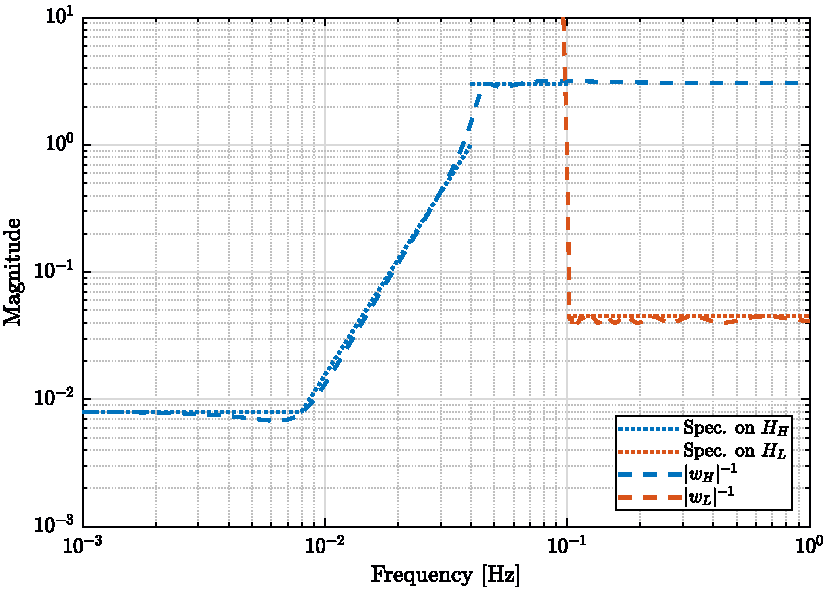
\includegraphics[scale=1]{figs/ligo_weights.pdf}
\caption{\label{fig:ligo_weights}
Specifications and weighting functions magnitudes}
\end{figure}

\subsection{\(\mathcal{H}_\infty\) Synthesis}
\label{sec:org58dd9fc}
\label{sec:ligo_results}
\(\mathcal{H}_\infty\) synthesis is performed using the architecture shown in Fig. \ref{eq:generalized_plant}.
The complementary filters obtained are of order \(27\).
In Fig. \ref{fig:comp_fir_ligo_hinf}, their bode plot is compared with the FIR filters of order 512 obtained in \cite{hua05_low_ligo}.
They are found to be very close to each other and this shows the effectiveness of the proposed synthesis method.

\begin{figure}[htbp]
\centering
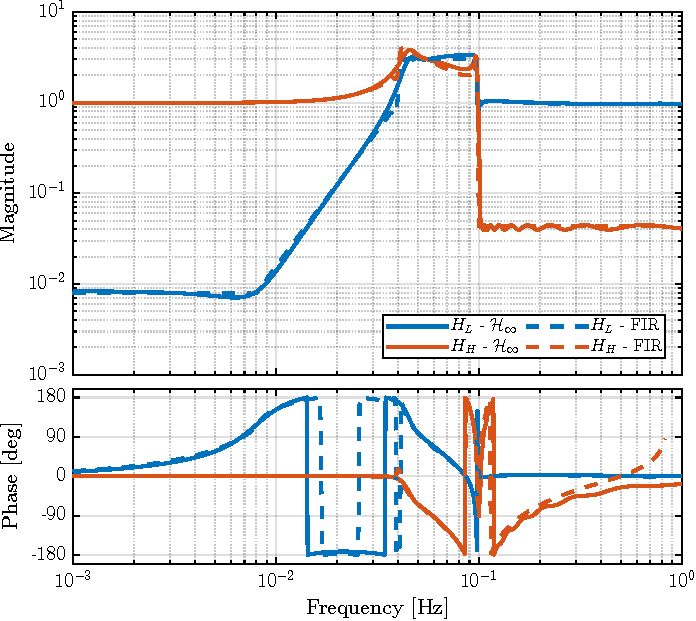
\includegraphics[scale=1]{figs/comp_fir_ligo_hinf.pdf}
\caption{\label{fig:comp_fir_ligo_hinf}
Comparison of the FIR filters (solid) designed in \cite{hua05_low_ligo} with the filters obtained with \(\mathcal{H}_\infty\) synthesis (dashed)}
\end{figure}

\section{Conclusion}
\label{sec:orgf6bb6aa}
\label{sec:conclusion}
This paper has shown how complementary filters can be used to combine multiple sensors in order to obtain a super sensor.
Typical specification on the super sensor noise and on the robustness of the sensor fusion has been shown to be linked to the norm of the complementary filters.
Therefore, a synthesis method that permits the shaping of the complementary filters norms has been proposed and has been successfully applied for the design of complex filters.
Future work will aim at further developing this synthesis method for the robust and optimal synthesis of complementary filters used in sensor fusion.

\section*{Acknowledgment}
\label{sec:org74249bf}
This research benefited from a FRIA grant from the French Community of Belgium.

\bibliography{ref}
\end{document}